\section{Screening Results}\label{sec:attribution}
\IfFileExists{tables/table3_observed.tex}{% Table 3: observed responses to the probes of Table 2 with the assigned class (cell sources: paper/tables/table2_NOTES.md,
% section "Table 3"). Input at the top of Sect. 6. Every number is a numbers.tex macro.
\begin{table}[t]
\caption{Observed response to each probe and assigned class, at the lone traps and the pair standoff. $x/y$: $x$ of $y$; $x$:$y$: discordant snapshots.}
\label{tab:observed}
\centering
\scriptsize
\setlength{\tabcolsep}{1pt}
\def\tl#1#2{\begin{tabular}[t]{@{}l@{}}#1\\#2\end{tabular}}%
\def\tll#1#2#3{\begin{tabular}[t]{@{}l@{}}#1\\#2\\#3\end{tabular}}%
\def\hd#1#2{\begin{tabular}[b]{@{}l@{}}#1\\#2\end{tabular}}%
\begin{tabular*}{\textwidth}{@{\extracolsep{\fill}}llllllllll@{}}
\toprule
Perturbation & Quench & Replay & $\Delta t$ & Push $\pm$ & Bias $\pm b$ & \hd{First}{exit} & \hd{Corrected;}{flag} & \hd{Replay}{sens.} & Class \\
\midrule
\multicolumn{10}{@{}l}{\emph{Lone traps}: force-coupled ORCA} \\
\quad RVO2 & \tl{frees}{\EtwoLKCThreeRVOFreed/\EtwoLKCThreeRVON} & \tl{identical,}{\TabThreeLKRvoReplayDis/\TabThreeLKRvoReplays} & \tl{flat;}{flat$^a$} & \tl{$+$\,\EtwoLKFrozenPlusFreed,}{$-$\,\EtwoLKFrozenMinusFreed} & n.a. & n.a. & \tl{persists;}{no} & no & \tl{Reshape,}{axial} \\
\quad legacy & \tl{frees}{\EtwoLKCThreePubFreed/\EtwoLKCThreeRVON} & \tl{changes,}{\RevAfiveXPoolLegacyReplayChanged/\RevAfiveXPoolLegacyReplays$^b$} & not run & as RVO2 & n.a. & n.a. & \tl{persists;}{no$^c$} & yes & \tl{Reshape,}{axial} \\
\tl{Noise $\sigma=$}{0.07\,m/s} & \tl{frees,}{matched$^d$} & \tl{disagree$^\dagger$,}{\TabThreeLKNoiseDisagree/\TabThreeLKNoiseSnaps} & \tl{$\ell=\PprotEllBA$;}{flat} & n.a. & n.a. & n.a. & n.a. & n.a. & Heat \\
\tll{ORCA}{velocity}{filter} & \tll{held;}{freed}{\VelLoneRvoK/\VelLoneN} & identical & not run & n.a. & n.a. & n.a. & \tl{persists;}{no} & no & \tl{at most}{Prevent} \\
\midrule
\multicolumn{10}{@{}l}{\emph{Pair standoff}: force-coupled ORCA} \\
\quad RVO2 & \tl{frees}{\PairRvoFreed/\PairN} & \tl{identical,}{\TabThreePairRvoReplayDis/\TabThreePairOrcaReplays} & not run & \tl{$+$\,\PairFrozenPlusFreed,}{$-$\,\PairFrozenMinusFreed} & n.a. & \tl{lower}{\TabThreePairRvoOrcaLower/\PairRvoFreed} & \tl{persists;}{no} & no & \tl{Reshape,}{axial$^e$} \\
\quad legacy & \tl{frees}{\PairPubFreed/\PairN} & \tl{identical,}{\TabThreePairPubReplayDis/\TabThreePairOrcaReplays} & not run & as RVO2 & n.a. & \tl{lower}{\PairPubLower/\PairPubFreed} & \tll{excess}{vanish;$^c$}{yes} & no & \tl{Reshape,}{axial$^e$} \\
\tl{Bias $+b^\ast$,}{legacy} & \tl{frees}{\PairBsPubFreed/\PairN} & \tl{identical,}{\TabThreePairBsPubReplayDis/\TabThreePairBsReplays} & not run & n.a. & \tl{$-b^\ast$: \PairBsPubMinusFreed,}{\PairBsPubRevA:\PairBsPubRevB$^f$} & \tll{side of $b^\dagger$:}{\PairBsPubHand/\PairBsPubN,}{\PairBsPubMinusUpper/\PairBsPubMinusFreed} & \tl{persists;}{no} & no & \tl{Reshape,}{lateral} \\
\bottomrule
\end{tabular*}
\par\smallskip\raggedright
$^\dagger$\,By construction. Flag: defect flag. n.a., not run, $\Delta t$ (per-step; $\sqrt{\Delta t}$-scaled noise): as in Table~\ref{tab:signatures}. Lone-trap counts: the \EtwoNLK\ lone keystones; filter: quenches of the screening set. $\ell$: Eq.~\eqref{eq:ell} pooled, $\beta_0=1.5$ ($\ell>0$: falls). First exit: lower, the member at $y<5$\,m; for the bias, the member favoured by the sign of $b$ ($+b^\ast$; $-b^\ast$). $^a$\,$|\ell|\le\EthreeCThreeLnRatioMax$ per snapshot. $^b$\,The \RevAfiveXPoolN\ second traps. $^c$\,Lone traps: freed set unchanged, replay changes vanish (replay sensitivity); the solver's flag comes from the pair standoff: \PairPubFreed\ freed fall to \PairRvoFreed\ (McNemar $p\PairPubRvoPRel$). $^d$\,Fraction-matched at $T=120$\,s at the lone keystones. $^e$\,Freed count solver-dependent; the constraint part opposes the drive part. $^f$\,Freed by $-b^\ast$, discordant with $+b^\ast$.
\end{table}
}{}

\subsection{The Lone Trap}\label{sec:att-lone}
\begin{figure}[t]
\centering
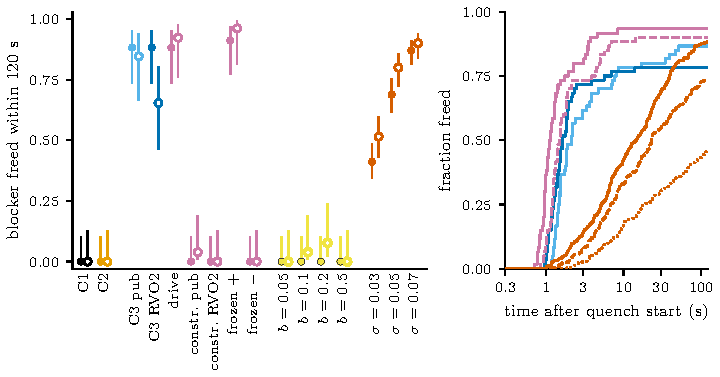
\includegraphics[width=\textwidth]{../figures/fig6_quench.pdf}
\caption{Left: blockers freed within 120\,s (filled, lone keystones; open, \EtwoNST\ of the \RevAfiveXPoolN\ second traps), 95\% cluster-bootstrap intervals over snapshots (none where every snapshot has the same outcome). Right: lone keystones freed against time, force-coupled ORCA (RVO2, solid) and noise $\sigma=0.07$\,m/s (dashed) with 95\% bands, others grey.}
\label{fig:quench}
\end{figure}
% generated by experiments/tables/make_tables45.py from paper/registry/*.yaml macros; do not edit
\begin{table}[t]
\caption{Per-step noise against force-coupled ORCA (RVO2), fraction-matched at the lone keystones and in whole runs.}
\label{tab:matched-noise}
\centering\scriptsize\setlength{\tabcolsep}{1pt}
\def\st#1#2{\begin{tabular}[t]{@{}c@{}}#1\\\relax#2\end{tabular}}%
\def\stl#1#2{\begin{tabular}[t]{@{}l@{}}#1\\\relax#2\end{tabular}}%
\def\hd#1#2{\begin{tabular}[b]{@{}c@{}}#1\\\relax#2\end{tabular}}%
\begin{tabular*}{\textwidth}{@{\extracolsep{\fill}}lcccccc@{}}
\toprule
Perturbation & Freed & $\Delta$ [95\%] & \hd{$\Delta$RMST (s)}{[95\%]} & Replay & \hd{$\Omega$}{(indep.)} & $\ell$ (pred.) \\
\midrule
\multicolumn{7}{@{}l}{\emph{Lone keystones: \EtwoNLK{} snapshots, $T=120$\,s}} \\
\stl{noise, 5 seeds}{$\sigma=0.07$\,m/s} & \EtwoLKNoiseCFreed{}/\EtwoLKNoiseCN{} & \st{$\RvAfiveLoneEtwoDiff{}$ [$\RvAfiveLoneEtwoDiffLo{}$, $\RvAfiveLoneEtwoDiffHi{}$]}{$p\RevAsevenLoneEtwoFreedPHolmRel{}$} & \st{$\PscrTimeLoneEtwoEff{}$ [$\PscrTimeLoneEtwoLo{}$, $\PscrTimeLoneEtwoHi{}$]}{$p\RevAsevenLoneEtwoTimePHolmRel{}$} & \TabThreeLKNoiseDisagree{}/\TabThreeLKNoiseSnaps{} & n.a. & \st{\PprotEllBA{} (\PprotEllBAPred{})}{$p\RevAsevenLoneEtwoEllPHolmRel{}$} \\
\stl{noise, 20 seeds}{$\sigma=\RunNOneSigma{}$\,m/s} & \RunNOneFreed{}/\RunNOneRunsN{} & \st{$\RvAfiveLoneNoneDiff{}$ [$\RvAfiveLoneNoneDiffLo{}$, $\RvAfiveLoneNoneDiffHi{}$]}{$p\RevAsevenLoneNoneFreedPHolmRel{}$} & \st{$\PscrTimeLoneNoneEff{}$ [$\PscrTimeLoneNoneLo{}$, $\PscrTimeLoneNoneHi{}$]}{$p\RevAsevenLoneNoneTimePHolmRel{}$} & \RevAsevenLoneNoneReplayDiscA{}/\EtwoNLK{} & \st{\RevAnineLKNHalfJ{} (\PscrLKNHalfEJ{})}{$p\RevAnineLKNHalfPRel{}$} & n.a. \\
\stl{force-coupled}{ORCA (RVO2)} & \EtwoLKCThreeRVOFreed{}/\EtwoLKCThreeRVON{} &  &  & \TabThreeLKRvoReplayDis{}/\TabThreeLKRvoReplays{} &  & $\PscrOrcaLnRatio{}$ \\
\midrule
\multicolumn{7}{@{}l}{\emph{Second traps: \RevAsixSTSnaps{} snapshots, $T=120$\,s}} \\
\stl{noise, 5 seeds}{$\sigma=0.07$\,m/s} & \RevAsixSTNoiseFreed{}/\RevAsixSTNoiseN{} & \st{$\RvAfiveSecondEtwoDiff{}$ [$\RvAfiveSecondEtwoDiffLo{}$, $\RvAfiveSecondEtwoDiffHi{}$]}{$p\RevAsevenSecondFreedPHolmRel{}$} & \st{$\PscrTimeSecondEff{}$ [$\PscrTimeSecondLo{}$, $\PscrTimeSecondHi{}$]}{$p\RevAsevenSecondTimePHolmRel{}$} & \RevAsixSTNoiseDisagree{}/\RevAsixSTSnaps{} & \st{\RevAsixSTJ{} (\RevAsixSTJInd{})}{$p=\RevAsixSTJIndP{}$} & not run \\
\stl{force-coupled}{ORCA (RVO2)} & \RevAsixSTOrcaFreed{}/\RevAsixSTOrcaN{} &  &  & \RevAsixSTOrcaReplayDis{}/\RevAsixSTOrcaReplays{} &  & not run \\
\midrule
\multicolumn{7}{@{}l}{\emph{Whole runs: \EsixN{} spawn seeds, $T=600$\,s}} \\
\stl{noise}{$\sigma^\ast=\EsixSigmaStar{}$\,m/s} & \EsixNoiseK{}/\EsixN{} & \st{$\RvAfiveWholeDiff{}$ [$\RvAfiveWholeDiffLo{}$, $\RvAfiveWholeDiffHi{}$]}{$p\RevAsevenWholeEsixFreedPHolmRel{}$} & \st{$\PscrTimeWholeEff{}$ [$\PscrTimeWholeLo{}$, $\PscrTimeWholeHi{}$]}{$p\RevAsevenWholeEsixTimePHolmRel{}$} & not run & \st{\RevAnineWholeEJ{} (\RevAnineWholeEEJ{})}{$p\RevAnineWholeEPRel{}$} & not run \\
\stl{force-coupled}{ORCA (RVO2)} & \EsixCThreeK{}/\EsixN{} &  &  & not run &  & not run \\
\bottomrule
\end{tabular*}
\par\smallskip
\parbox{\textwidth}{\scriptsize Freed: runs freed by $T$ (noise), snapshots (force-coupled ORCA), runs completed (whole runs). $\Delta$: freed fraction, noise minus force-coupled ORCA. $\Delta$RMST: difference of the mean time to free, capped at $T$. Replay: snapshots whose seeds disagree (noise, by construction) or whose $10^{-9}$\,m replay changes the outcome (force-coupled ORCA). $\Omega$: Jaccard index of the unresolved sets (noise: freed in fewer than half the seeds); in parentheses, for independent sets. $\ell$: Eq.~\eqref{eq:ell} pooled over the \EthreeN{} snapshots of the time-step set, noise at $\beta=1.5$ (prediction). Intervals are unadjusted. $p$ beside $\Delta$, $\Delta$RMST and $\ell$: paired test, Holm-adjusted over the probes of the comparison (lone keystones 4: $\Delta$, replay, $\Delta$RMST and either $\ell$ or outcome identity; second traps 3; whole runs 4: $\Delta$, outcome identity, $\Delta$RMST, final-state class). $p$ beside $\Omega$: hypergeometric, unadjusted. n.a.: not applicable; not run: probe not run on this set.}
\end{table}

%
On the screening set a blocker is freed if it exits within $T=120$\,s (Fig.~\ref{fig:quench}; Tables~\ref{tab:observed} and~\ref{tab:matched-noise}).

\subsubsection{Force-Coupled ORCA's Parts at the Lone Keystone.}
The drive part alone frees the same lone keystones as force-coupled ORCA with either solver. By Eq.~\eqref{eq:identity} the drive plus drive part is the SFM with relaxation time $\tau'$. The SFM with $\tau'$, quenched from each snapshot, frees the same \RevAoneLoneFreed\ of \RevAoneLoneN\ lone keystones and \RevAoneSecondFreed\ of \RevAoneSecondN\ second traps (discordant \RevAoneDiscA:\RevAoneDiscB). The constraint part alone frees \EtwoLKConstrRVOFreed\ (RVO2) and \EtwoLKConstrPubFreed\ (legacy). The rest-drive push frees \EtwoLKFrozenPlusFreed\ towards the door, earlier than force-coupled ORCA (RVO2) ($\Delta$RMST $\RevAsevenPushLoneTimeEff$\,s, Holm $p\RevAsevenPushLoneTimePHolmRel$), and \EtwoLKFrozenMinusFreed\ away. SFM and SFM+TTC free none of the \EtwoNAll\ snapshots of the screening set. Force-coupled ORCA (RVO2) holds the blocker where the stuck-alone margin with its rest drive added stays positive (ROC area \EtwoLKMarginAUC). Elsewhere its rest drive removes the fixed point, and it frees the blocker through this rest force.

\subsubsection{Fraction-Matched Noise.}
Per-step noise at $\sigma=0.07$\,m/s (five seeds) and $\sigma=\RunNOneSigma$\,m/s (20 seeds) is fraction-matched to force-coupled ORCA (RVO2) at $T=120$\,s. At $\sigma=0.07$\,m/s the median $\beta$ at the lone keystone is \RevAthreeSevenMed, so this noise frees deadlocks by fluctuations (Sect.~\ref{sec:escape}).
%C2: A5 A6 equivalence margin for the freed-fraction match; whether the lone-keystone Delta intervals of Table 4 lie inside it
The 20-seed runs leave \RevAnineLKNHalfA\ snapshots unresolved, all among the \RevAnineLKNHalfB\ that force-coupled ORCA (RVO2) holds; five seeds misclassify \RevAnineMisclass\ on average. Two halves of the noise seeds overlap as much as noise and force-coupled ORCA (RVO2) do ($\Omega=\RunNOneJNoiseNoise$ and \RevAnineLKNHalfJ), so overlap does not separate them. Replay separates them by construction: the noise seeds disagree on \RevAsevenLoneEtwoReplayDiscA\ snapshots, the replays of force-coupled ORCA (RVO2) on \TabThreeLKRvoReplayDis\ of \TabThreeLKRvoReplays.

The time step separates them as well (\EthreeN\ snapshots of the time-step set; Fig.~\ref{fig:escape}(c), Table~\ref{tab:matched-noise}): the escape rate under per-step noise follows Eq.~\eqref{eq:ell}, $\sqrt{\Delta t}$-scaled noise does not, and force-coupled ORCA (RVO2) frees the same snapshots at every $\Delta t$. The lateral bias frees no lone keystone at any $b$ (upper Wilson bound \EtwoMaxBiasUpperLK).

\subsubsection{Second Trap and the Legacy Solver.}
At the second trap the constraint part opposes the drive part: a trapped neighbour stands abreast of the blocker across the door axis (\CtwsixAbreastN\ of \CtwsixN\ one-neighbour snapshots), and its half-plane cancels a median \StHeldCancel\ of the drive while the blocker moves. Adding \RevAfiveXNewN\ random snapshots to the screening set's \RevAfiveXEtwoN\ gives \RevAfiveXPoolN\ second traps; both groups respond alike to every perturbation (Holm $p\RevAfiveXVsEtwoMinPHolmRel$). On all of them the drive part frees \RevAfiveXPoolDriveFreed\ blockers and force-coupled ORCA (RVO2) frees \RevAfiveXPoolOrcaFreed\ (McNemar $p\RevAfiveXPoolDriveOrcaPDisp$). The SFM quench frees \RevAfiveXPoolSFMFreed; each still moved below the deadlock criterion's 0.01\,m/s at the snapshot. Noise at $\sigma=0.07$\,m/s frees more blockers than force-coupled ORCA (RVO2) and is not fraction-matched here ($\Delta=\RevAfiveXPoolNoiseOrcaEff$ [$\RevAfiveXPoolNoiseOrcaLo$, $\RevAfiveXPoolNoiseOrcaHi$]).

The legacy solver is the authors' earlier solver~\cite{gang2026}. For a leg of the velocity obstacle with unit direction $\hat{\mathbf d}$ it takes the half-plane normal along $\mathbf u=(\mathbf v_{\rm rel}\cdot\hat{\mathbf d})\,\hat{\mathbf d}-\mathbf v_{\rm rel}$, the change of the relative velocity onto the leg; RVO2 takes the leg direction rotated by $90^\circ$:
\begin{equation}\label{eq:legnormal}
\mathbf n_{\rm legacy}=\frac{\mathbf u}{|\mathbf u|}=-\operatorname{sgn}(\mathbf v_{\rm rel}\cdot\mathbf n_{\rm RVO2})\,\mathbf n_{\rm RVO2},\qquad \mathbf n_{\rm RVO2}=(-\hat d_y,\,\hat d_x).
\end{equation}
The two normals agree while the relative velocity lies inside the velocity obstacle; outside it the legacy half-plane is inverted. Its $10^{-9}$\,m replays change the outcome in \EtwoReplayCThreePubFlips\ of \EtwoReplayN\ on the screening set and \RevAfiveXPoolLegacyReplayChanged\ of \RevAfiveXPoolLegacyReplays\ on the \RevAfiveXPoolN\ second traps, those of the RVO2 solver in none. The blocker jitters at \PscrCreepSpeedMin--\RevAthirteenCreepSpeedMax\,m/s (net axial drift $\RevAthirteenCreepDriftMin$ to $+\RevAthirteenCreepDriftMax$\,mm/s). Two replays diverge where a leg normal flips sign (\FixAfourDiscLegFlip\ of \FixAfourDiscN\ first divergences), and the exit then shifts by up to \PscrReplayPubMaxDt\,s. The legacy solver frees blockers through its rest force as the RVO2 solver does. Its replay flips vanish with the RVO2 solver, so it carries the defect flag.

\subsection{Whole Runs}\label{sec:att-whole}
Noise fraction-matched at $T=600$\,s differs from force-coupled ORCA (RVO2) in time to completion and final state. Half the runs with per-step noise complete at $\sigma_{50}=\EfiveSigmaFifty$ [\FixAsixSigFiftyClLo, \FixAsixSigFiftyClHi]\,m/s (\EfiveN\ runs per level); the fit meets the completion of force-coupled ORCA (RVO2) at $\sigma^\ast=\EsixSigmaStar$\,m/s. The unresolved sets of noise and force-coupled ORCA (RVO2) overlap more than independent sets ($\Omega=\RevAnineWholeEJ$ against \RevAnineWholeEEJ, hypergeometric $p\RevAnineWholeEPRel$; Table~\ref{tab:matched-noise}).
%C2: A5 A6 equivalence margin for the whole-run completion match; whether the whole-run Delta interval of Table 4 lies inside it

Force-coupled ORCA (RVO2) is faster on all \EsixPairedCThreeFaster\ seeds where both complete (median lead \EsixPairedDelay\,s). The final states at 600\,s differ in class (Holm $p\RevAsevenWholeEsixClassPHolmRel$). Force-coupled ORCA's \EsixCThreeFailRest\ failures at rest are lone keystones, and \EsixCThreeMovingSecond\ of its \EsixCThreeFailMoving\ moving failures hold a second trap. Noise failures never come to rest; they hold \EsixNoiseLone\ lone keystones, \EsixNoiseSecond\ second traps and \EsixNoiseCollective\ group standoffs. The survival function of noise stalls (at least 10\,s without an exit) lies within \PscrStallMaxDiff\ of its prediction from the \EsixBarrierN\ barriers of the barrier set, $k_{\rm B}T_{\rm eff}(\sigma^\ast)$ and the attempt frequency of Sect.~\ref{sec:escape}, with no parameter fitted to the whole-run data. This prediction extrapolates the Arrhenius law below $\beta=1.5$: at $\sigma^\ast$ the median $\beta$ is \RevAthreeStarMed\ and \RevAthreeStarBelowOneK\ of \RevAthreeBarN\ barriers have $\beta<1$, so the noise frees whole-run deadlocks by fluctuations.

\subsection{The Pair Standoff}\label{sec:att-pair}
\begin{figure}[t]
\centering
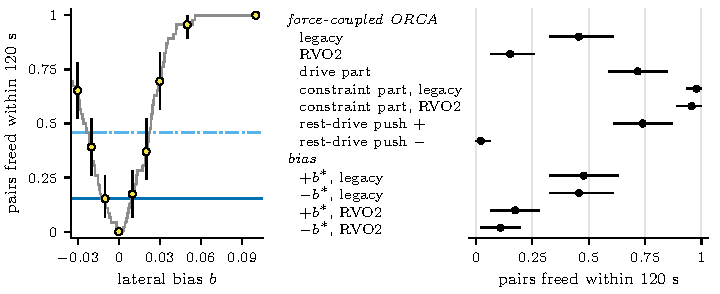
\includegraphics[width=\textwidth]{../figures/fig7_pair.pdf}
\caption{Pair standoffs freed within 120\,s against the lateral bias $b$ (left; grey steps, static threshold prediction; force-coupled ORCA, legacy dash-dot, RVO2 solid) and per perturbation (right), 95\% bootstrap intervals over snapshots (none where every snapshot has the same outcome).}
\label{fig:pair}
\end{figure}
% generated by experiments/tables/make_tables45.py from paper/registry/*.yaml macros; do not edit
\begin{table}[t]
\caption{Lateral bias $+b^\ast$ fraction-matched to force-coupled ORCA with the same solver at the pair standoff.}
\label{tab:matched-bias}
\centering\scriptsize\setlength{\tabcolsep}{1pt}
\def\st#1#2{\begin{tabular}[t]{@{}c@{}}#1\\\relax#2\end{tabular}}%
\def\stl#1#2{\begin{tabular}[t]{@{}l@{}}#1\\\relax#2\end{tabular}}%
\def\hd#1#2{\begin{tabular}[b]{@{}c@{}}#1\\\relax#2\end{tabular}}%
\begin{tabular*}{\textwidth}{@{\extracolsep{\fill}}lcccccc@{}}
\toprule
Perturbation & Freed & $\Delta$ [95\%] & \hd{$\Delta$RMST (s)}{[95\%]} & Replay & \hd{$\Omega$}{(indep.)} & \hd{First exit}{below axis} \\
\midrule
\multicolumn{7}{@{}l}{\emph{Legacy solver: \PairN{} pair standoffs, $T=120$\,s}} \\
\stl{bias}{$+b^\ast_{\rm legacy}=\PscrPairBstarPub{}$} & \PairBsPubFreed{}/\PairN{} & \st{$\PscrPairPubDiff{}$ [$\PscrPairPubDiffLo{}$, $\PscrPairPubDiffHi{}$]}{$p\RevAsevenPairPubFreedPHolmRel{}$} & \st{$\PscrTimePairPubEff{}$ [$\PscrTimePairPubLo{}$, $\PscrTimePairPubHi{}$]}{$p\RevAsevenPairPubTimePHolmRel{}$} & \TabThreePairBsPubReplayDis{}/\TabThreePairBsReplays{} & \st{\RevAninePairPubJ{} (\RevAninePairPubEJ{})}{$p\RevAninePairPubPRel{}$} & \st{\PairBsPubHand{}/\PairBsPubN{}}{$p\RevAsevenPairPubHandPHolmRel{}$} \\
\stl{force-coupled}{ORCA (legacy)} & \PairPubFreed{}/\PairN{} &  &  & \TabThreePairPubReplayDis{}/\TabThreePairOrcaReplays{} &  & \PairPubLower{}/\TabThreePairPubOrcaN{} \\
\midrule
\multicolumn{7}{@{}l}{\emph{RVO2 solver: \PairN{} pair standoffs, $T=120$\,s}} \\
\stl{bias}{$+b^\ast_{\rm RVO2}=\PairBstarRvo{}$} & \PairBsRvoFreed{}/\PairN{} & \st{$\PscrPairRvoDiff{}$ [$\PscrPairRvoDiffLo{}$, $\PscrPairRvoDiffHi{}$]}{$p\RevAsevenPairRvoFreedPHolmRel{}$} & \st{$\PscrTimePairRvoEff{}$ [$\PscrTimePairRvoLo{}$, $\PscrTimePairRvoHi{}$]}{$p\RevAsevenPairRvoTimePHolmRel{}$} & \TabThreePairBsRvoReplayDis{}/\TabThreePairBsReplays{} & \st{\RevAninePairRvoJ{} (\PscrPairRvoEJ{})}{$p\RevAninePairRvoPLeRel{}$$^\dagger$} & \st{\TabThreePairRvoHand{}/\TabThreePairRvoHandN{}}{$p\RevAsevenPairRvoHandPHolmRel{}$} \\
\stl{force-coupled}{ORCA (RVO2)} & \PairRvoFreed{}/\PairN{} &  &  & \TabThreePairRvoReplayDis{}/\TabThreePairOrcaReplays{} &  & \TabThreePairRvoOrcaLower{}/\TabThreePairRvoOrcaN{} \\
\bottomrule
\end{tabular*}
\par\smallskip
\parbox{\textwidth}{\scriptsize Columns as in Table~\ref{tab:matched-noise}; $\Omega$ compares the freed sets. First exit below axis: freed standoffs first left by the member at $y<5$\,m, below the door axis. Holm family per solver: 5 probes ($\Delta$, replay, outcome identity, $\Delta$RMST, first exit). $^\dagger$$\Omega=0$: $p$ of an overlap this small or smaller.}
\end{table}

%
Every held standoff under force-coupled ORCA still moves at 120\,s (Fig.~\ref{fig:pair}; \RevAfifteenPairRvoMoving\ of \RevAfifteenPairRvoHeld\ RVO2, \RevAfifteenPairPubMoving\ of \RevAfifteenPairPubHeld\ legacy), so results are freed fractions at $T=120$\,s.

\subsubsection{Force-Coupled ORCA's Parts at the Pair.}
Force-coupled ORCA frees \PairPubFreed\ of the \PairN\ standoffs with the legacy solver and \PairRvoFreed\ with the RVO2 solver (McNemar $p\PairPubRvoPRel$). Its drive part alone frees \PairDriveFreed. The rest-drive push frees \PairFrozenPlusFreed\ towards the door and \PairFrozenMinusFreed\ away. At rest the half-plane against the partner binds at all \RevAelevenPairBinds\ members, and the constraint part points laterally away from it with \RevAelevenRatioMin--\RevAelevenRatioMax\ of the drive's magnitude. This rest field is not a gradient (Jacobian asymmetry \PscrJacAsymMin--\RevAelevenJacAsymMax), so the stability argument of Sect.~\ref{sec:rest} does not cover force-coupled ORCA at the pair. Alone, the constraint part frees \PairConsPubFreed\ (legacy) and \PairConsRvoFreed\ (RVO2). Added to the drive part, it cancels the drive's squeeze towards the axis, so force-coupled ORCA (RVO2) frees fewer standoffs than the drive part alone ($p\PairDriveRvoPRel$). Of the \RevAelevenPairDisc\ standoffs that the drive part frees and force-coupled ORCA (RVO2) holds, the rest field accounts for \RevAelevenPairDiscStatic; the others and the solver difference arise in motion, where the half-plane turns towards the door.

\subsubsection{Fraction-Matched Lateral Bias.}
The bias $b^\ast$ is read off the thresholds $b_f$ of the same snapshots, so it is an in-sample estimate and reproduces each solver's freed fraction at $T=120$\,s by construction.
%C2: A5 A6 split-half result for b*; equivalence margin and whether each interval lies inside it
With either solver its freed set overlaps that of force-coupled ORCA as much as independent sets would (Table~\ref{tab:matched-bias}). Handedness separates the bias from force-coupled ORCA. The member below the door axis, favoured by $b>0$, exits first in every standoff the bias frees. Under force-coupled ORCA it exits first in \PairPubLower\ of \PairPubFreed\ freed standoffs (legacy) and \TabThreePairRvoOrcaLower\ of \PairRvoFreed\ (RVO2). The reversed bias frees \PairBsPubMinusFreed\ (legacy) and \PscrPairBsRvoMinusFreed\ (RVO2) standoffs, with the member above the axis first in all, and frees different ones from $+b^\ast$ (discordant \PairBsPubRevA:\PairBsPubRevB, legacy).

\subsection{The ORCA Velocity Filter}\label{sec:velorca}
The ORCA velocity filter (Eq.~\eqref{eq:velorca}) frees no deadlock. At a snapshot no pair is in contact, so every half-plane admits $\mathbf v=\mathbf 0$ with slack at least $(d_{ij}-r_{ij})/2\tau_h$; the filter returns $\mathbf v=\mathbf 0$ and adds no rest drive. With either solver it frees \VelLoneRvoK\ of \VelLoneN\ lone-trap and \VelPairRvoK\ of \VelPairN\ pair quenches. On another \VelWholeN\ spawn seeds \VelWholeK\ run completes under the filter and \VelWholeSfmK\ under SFM, against \VelWholeForceK\ under force-coupled ORCA (McNemar $p\VelWholeForcePRel$). All \VelWholeFail\ failures end at rest in states that SFM also holds, so the filter acts at most while the crowd moves.
